%!TEX root = ../thesis.tex

\chapter{Evaluation}
\label{sec:evaluation}

In this section we will evaluate our set design goals and discuss our implementation in detail.
Further we will analyze our design decisions.
Where applicable the functional and non-functional requirements will be validated.

\section{Infrastructure}

This section follows the same structure as used in the previous Chapter~\ref{sec:infrastructure}.
The infrastructure consists of the server part and the local part.
Both are evaluated in the following sections.
In the end the deployed infrastructure is evaluated in a field test.

\subsection{Server Infrastructure}

\subsubsection{Design Goals}

Section~\ref{sec:server_infrastructure_design_goals} lists the design goals defined for this project part.
Each design goal will be evaluated in a separate paragraph below.

\paragraph{Modularity and Extensibility} Django emphasizes reusability of components.
This solid background allows us to clearly separate different concerns to achieve modularity.
Further the distinct components simplify application extensions by easily adding new resources, representations, views or URLs.

\paragraph{Usability} In order for a developer to be able to familiarize himself with a new API it is important to provide clear documentation and a platform to use the API.
The browsable API as described in Section~\ref{sec:server_infrastructure_restful_api} provides both.
It allows a developer to interactively explore the resource structure by navigating via the displayed URLs.
The browsable API also provides easy interaction possibilities to create, read, update and delete resources.
Further the API describes the supported access methods when requesting a particular resource.
One of these HTTP methods named \emph{OPTIONS} shows the accessible fields, their types and other useful meta information for interacting with the API.


\paragraph{Testability}

The modular program structure and the chosen Django framework support the creation and automatized execution of software tests.
These automatized tests are continuously executed on a hosted service and show that the tests run regularly and successfully.


\subsubsection{Design Decisions}

During the system implementation a few design decisions were chosen and will be evaluated in the following paragraphs.

\paragraph{Nested URL schema}

The model hierarchy is represented using a nested URL schema.
This schema suits the model structure in tree form and induces good readable URLs.
Django is designed for flat URLs but is still flexible enough to support the design decision of implementing a nested URL schema for resources access.

\paragraph{Resource identifier as the first field}

Within the resource representation the resource identifier is always the first field.
This allows to easily recognize the identifier within resource representations and especially within nested resource representation.

\paragraph{Resource referencing}

Resources are referenced by including their representation.
This design decision improves the usability of the API, as related resources are shown in their full representation and also allows to reduce the number of required requests.
In contrast collections are referenced via their URL.
This is necessary to limit the representation size and avoid infinite recursions.
For example in a parent-child relationship the child representation contains the representation of its parent.
The parent representation itself contains the collection representation of its children.
Therefore the collection representation cannot contain the full representations of its resources.

\paragraph{Identification of URL fields}

Fields representing a URL are identified by the name \highlight{url} or the suffix \highlight{\_url}.
This design decision facilitates the recognition of hyperlinks which also allows an automatized navigation through the API.



\subsection{Local Deployment}


%\subsubsection{Design Goals}

The following section will evaluate each of the design goals defined in Section~\ref{sec:local_infrastructure_design_goals}.
Please note that the reliability is evaluated separately in a field test described in Section~\ref{sec:evaluation_field_test}.

The local infrastructure section is about the implementation part done on the residential communication gateway.
Therefore the following paragraphs focus on the evaluation of software running on the Raspberry computer.

\subsubsection{Performance}
% for low computational effort and power consumption on embedded systems.

The system performance depends on two aspects.
First, the software part.
The programming language \emph{Python} was chosen at it is suitable for developing on embedded hardware with possibly long-running input/output operations.
Another important component is the system design of independent scripts triggered by a scheduler. % \emph{cron}.
Second, the embedded hardware part.
The chosen hardware needs to be powerful enough to run the developed software implementation.

For evaluation of the ratio between required software performance and provided hardware performance the CPU load is monitored.
We use the \emph{sar} command from the \emph{apt-get} package \emph{sysstat} to analyze the average CPU utilization.
Over a period of seven days of regular system runtime the average CPU load was 0.28 percent.
This indicates that the hardware is powerful enough to run the designed software implementation.


\subsubsection{Robustness}
% to let the system behave reasonably in presence of failures, especially connection problems.

We defined robustness to be the ability of the system to behave reasonably in the presence of failures, especially connection problems.
The local communication gateway is designed as two independent tasks.
The first task is the retrieval and storage of the temperature data and the application of the defined schedule.
The second task is the synchronization of the local data storage with the remote Web server.
This design splits the responsibility of the local communication system into two simpler separated tasks with a clearly defined interface, the local data storage.
In the presence of a failure only one of the two tasks is affected whereas the other task is still able fulfill its purpose.

For example in the event of a temporary Internet connection disruption the system will keep operating the last downloaded heating schedule and store the temperature history.
After the disruption the local data storage is synchronized and the system continues to operate on the most actual settings.

Another failure scenario would be the temporary disconnection of a wireless thermostat.
In such a case the non-affected thermostats are still functional and the heating schedule of all thermostats is kept in sync with the Web server.
As soon as the system reestablishes the connection to the affected thermostat the system continues to work as planned.
In the meantime neither the properly operating thermostats nor the synchronization of all thermostats' heating schedules is impaired.







\subsubsection{Interoperability}
% to cooperate with other distributed systems

We define interoperability as the system's ability to cooperate with other distributed systems.
The whole infrastructure is designed to communicate according to recognized open standards and architectural styles such as \emph{Constrained Application Protocol (CoAP)}, \emph{Hypertext Transfer Protocol (HTTP)}, \emph{Internet Protocol (IP)}, \emph{JavaScript Object Notation (JSON)} and \emph{Representational State Transfer (REST)}.
This way the developed infrastructure is able to cooperate with other distributed system via the defined interfaces.


\subsection{Field test}
\label{sec:evaluation_field_test}
% for a high probability that the system operates as expected

In order to check the reliability of the infrastructure in a real world scenario the system has been deployed in a residential home.
Previous work in this area compared the defined room temperatures with the actual room temperatures to conclude on the proper work of a heating system\cite{eigenmann2012opportunisticSensing}.
Due to the summer season and the according temperatures this evaluation is not possible for this project.
Instead we focus on the communication between the wireless thermostats, the local communication gateway and the remote server to evaluate the reliability.
The main data sources for our analysis are the data storages on the local communication gateway, the database on the remote Web server and the generated log files on both parts of the infrastructure.
We present our analysis of two different time spans.

\subsubsection{First evaluation}

In the following we analyze the data from the time span of August 2015.

\paragraph{Local data storage analysis}

% 2969 Rows returned from: SELECT * FROM heating_temperature
% WHERE timestamp BETWEEN '2015-08-01' AND '2015-09-01' (took 12ms)

% SELECT strftime('%d', timestamp), COUNT(*), * FROM heating_temperature
% WHERE timestamp BETWEEN '2015-08-01' AND '2015-09-01'
% GROUP BY strftime('%d', timestamp)
We start with the analysis of the local data storage.
It is used to cache the temperature readings and other meta data read from the thermostats before it is send to the remote server.
The local communication gateway queries the thermostats every 15 minutes, i.e. 96 times a day.
The maximal number of temperature measurements and meta entries would therefore be 2976 for the whole month of August.
The local data storage contains 2969 of these recorded temperature measurements in this date range, resulting in a coverage of 99.76 percent.
The coverage of the meta data is even slightly higher.
Please see Table~\ref{table:evaluation_local_database_coverage} for the full coverage data.

\begin{table}[h]
	\begin{center}
		\begin{tabular}{ l | r r r }
			\toprule
			Local Database entries & Maximal count & Actual count & Coverage \\
			\midrule
			Temperature			& 2976 & 2969 & 99.76 \% \\
			%			Server temperature entries	& 2976 & 2969 & 99.76 \%
			Meta data			& 2976 & 2970 & 99.80 \% \\
			\bottomrule
		\end{tabular}
		\caption{Retrieved temperature measurements and meta entries in a real world deployment in August 2015.}
		\label{table:evaluation_local_database_coverage}
	\end{center}
\end{table}

\paragraph{Local log file analysis}

Each log entry has a severity level indicating the impact of a logged event on system stability and functionality.
We evaluated these severity levels and their according log messages to analyze the system behavior as well as to identify potential problems.

There are almost a hundred thousand log entries which reveal a few interesting facts.
The rate of successful CoAP requests varies highly depending on the queried resource.
See the Table~\ref{table:evaluation_coap_requests} for the full data.
The requests to the operation mode and target temperature resources failed much more often than queries to other resources.
Especially the PUT requests fail in more than 72 percent.
Therefore the correct functioning could not be guaranteed in this time range.

\begin{table}[h]
	\begin{center}
		\begin{tabular}{ l | r r r r }
			\toprule
			CoAP request	& Total	& Success	& Timeouts	& Success rate \\
			\midrule
			GET /debug/heartbeat	& 2975	& 2970	& 5	& 99.8 \% \\
			GET /sensors/temperature	& 2975	& 2969	& 6	& 99.8 \% \\
			GET /set/mode	& 2975	& 2970	& 5	& 99.8 \% \\
			PUT /set/mode	& 803	& 181	& 622	& 22.5 \% \\
			GET /set/target	& 2975	& 1216	& 1758	& 40.9 \% \\
			PUT /set/target	& 2698	& 741	& 1957	& 27.5 \% \\
			\bottomrule
		\end{tabular}
		\caption{Analyzed CoAP requests in August 2015.}
		\label{table:evaluation_coap_requests}
	\end{center}
\end{table}

We discovered the following potential issues:
\begin{itemize}
	\item The applied target mode ``manual target'' often got overridden by ``radio target''.
	\item There are many CoAP requests sent closely following each other. This may overwhelm the low power devices.
	\item There is an invalid temperature value in the heating schedule which is rejected by the thermostat. 1244 out of 1957 time outs are related to this invalid value.
\end{itemize}

We address these potential issues in the next section and describe appropriate improvements.

Another interesting fact is the handling of temporary losses of Internet connection.
Due to an Internet modem failure and the necessary replacement actions, the residence local network was offline for about 48 hours.
During this time the local gateway kept communicating with the wireless thermostat to operate the schedule and log the measured temperatures.
After reestablishing the Internet access all temperature measurements that have not yet been uploaded were pushed to the Web server.
It took about 56 seconds to upload the missing 192 measurements.
During and after the whole external incident the system reacted and worked as planned.

\paragraph{Server analysis}


The server logs all received HTTP requests into a log file.
Each log entry contains the requested URL, the HTTP method and the HTTP response code.
In the chosen time span there were 2969 successful POST requests each adding a single temperature measurement.
This matches the number of temperature entries in the storage on the local communication gateway and in the server database and shows that all temperature measurements were successfully transmitted and persisted on the server.
In contrast the server log file shows that there is a known problem with the storage of meta data causing the related HTTP requests to be rejected.
The local communication gateway makes five attempts until it marks an entry as failed.
However no data is lost since marked entries are not deleted from the gateway database.


% 2969 Rows returned from: SELECT * FROM smart_heating_temperature WHERE thermostat_id = "04B753B9212580"
% AND datetime BETWEEN '2015-08-01' AND '2015-09-01' (took 23ms)

%The analysis of the server database is similar to the analysis of the local database.
%In the evaluated time span there are 2969 temperature entries out of 2976 possible measurements.
%These are the same entries as on the local communication gateway.

\subsubsection{Second evaluation}

After the long-term field test another test was set up to evaluate the effects of further improvements.
In this second evaluation we focus our analysis on the CoAP communication between the gateway and the thermostat.
We discovered a high failure rate for both PUT requests in the previous evaluation and tried to address this issue with several corrections.

We suspect the low power devices to may be overwhelmed by too many closely following requests.
Therefore we drastically limit the number of request to one within three seconds.
Additionally we repeat certain unanswered requests up to three times until a response is received.
Furthermore the heating schedule is cleaned from the invalid value and the updated server does no longer accept temperatures that are not supported by the deployed thermostat.

The revised implementation is deployed to the local communication gateway and monitored.
Due to time constraints we could not collect the same amount of data as in the first evaluation.
The following analyzed data is based on a time span of 13.5 days.
See Table~\ref{table:evaluation_coap_requests2} for the complete data.

\begin{threeparttable}[htbp]
	\centering
	\begin{tabular}{ l | r r r r r }
		\toprule
		CoAP request	& Total	& Unique\tnote{\textdagger}	& Success	& Timeouts	& Success rate \\
		\midrule
		GET /debug/heartbeat	& 1300	& 1300	& 1277	& 23	& 98.2 \% \\
		GET /sensors/temperature	& 1300	& 1300	& 1280	& 0	& 98.5 \% \\
		GET /set/mode	& 1300	& 1300	& 1286	& 14	& 98.9 \% \\
		PUT /set/mode	& 1	& 1	& 0	& 0	& - \\
		GET /set/target	& 1779	& 1300	& 1272	& 507	& 97.8 \% \\
		PUT /set/target	\tnote{\textasteriskcentered} & 49	& 49	& 6	& 40	& 12.2 \% \\
		\bottomrule
	\end{tabular}
	\begin{tablenotes}
		\footnotesize{
			\item[\textdagger] Number of requests not considering repetitions.
			\item[\textasteriskcentered] Also see the paragraph \emph{Hardware issues} for details.
		}
	\end{tablenotes}
	\caption{Analyzed CoAP requests of the second evaluation.}
	\label{table:evaluation_coap_requests2}
\end{threeparttable}

The curbed request rate and the repetition of timed out \highlight{GET /set/target} requests enhanced their success rate radically.
The success rate increased from 40.9 percent to 97.8 percent.
Interestingly the repetition of failed \highlight{PUT /set/target} requests did not improve its success rate.
This adjustment was separately tested but then discarded.
However the total number of PUT requests fell intensively due to the improved results of GET requests and the way of implementation, as PUT requests are only submitted if the desired values is not already set.
The data shows the resource \highlight{/set/mode} only required a single write.
Further analysis suggests that the mode is also set when writing the target and does not need to be set separately.
The remaining GET requests seem not to be affected by the improvements.

\paragraph{Hardware issues}

A closer look at the data indicates that the timed out \highlight{PUT /set/target} requests did still make an impact.
Although when the gateway did not receive a response, the requested target temperature is returned by the subsequent GET query.
Further inspection indicate that there is a general problem with the deployed Honeywell thermostat probably caused by weak hardware communication interfaces (UART) or the upgraded open source firmware OpenHR20.


\section{Mobile App}
\label{sec:eval_mobile_app}

\subsection {Use cases coverage}
Our mobile control application covers most of the use cases introduced in Section \ref{sec:use_cases} adequately. As shown later in some cases we decided to either leave the feature out for simplicity's sake or because it was out of scope for this lab project.

\begin{enumerate}
\item \textbf{Use Case: User wants to install the system}

Covered by the welcome view: The user can easily setup the system using the NFC tags distributed on the raspberry pi and the thermostats with the help of the information displayed on the application.
\item \textbf{Use Case: User feels cold}

Covered by the detail view: The user can adjust the temperature of the room he is currently in using the slider in the detail view.
\item \textbf{Use Case: User wants to save money}

Indirectly covered: The user can choose to set the temperatures lower than usual in order to save money.
\item \textbf{Use Case: User wants to add a room to an existing system}

Covered by the home view: The user can simply add a room using the menu in the upper righthand corner or the button at the bottom of the screen.
\item \textbf{Use Case: User wants to add a thermostat to a room in the system}

Covered by the detail view: The user can add a new thermostat to the currently selected room by simply scanning its NFC tag.
\item \textbf{Use Case: User feels hot}

Covered by the detail view: The user can adjust the temperature of the room he is currently in using the slider in the detail view.
\end{enumerate}

\begin{figure} [h]
	\begin{center}
		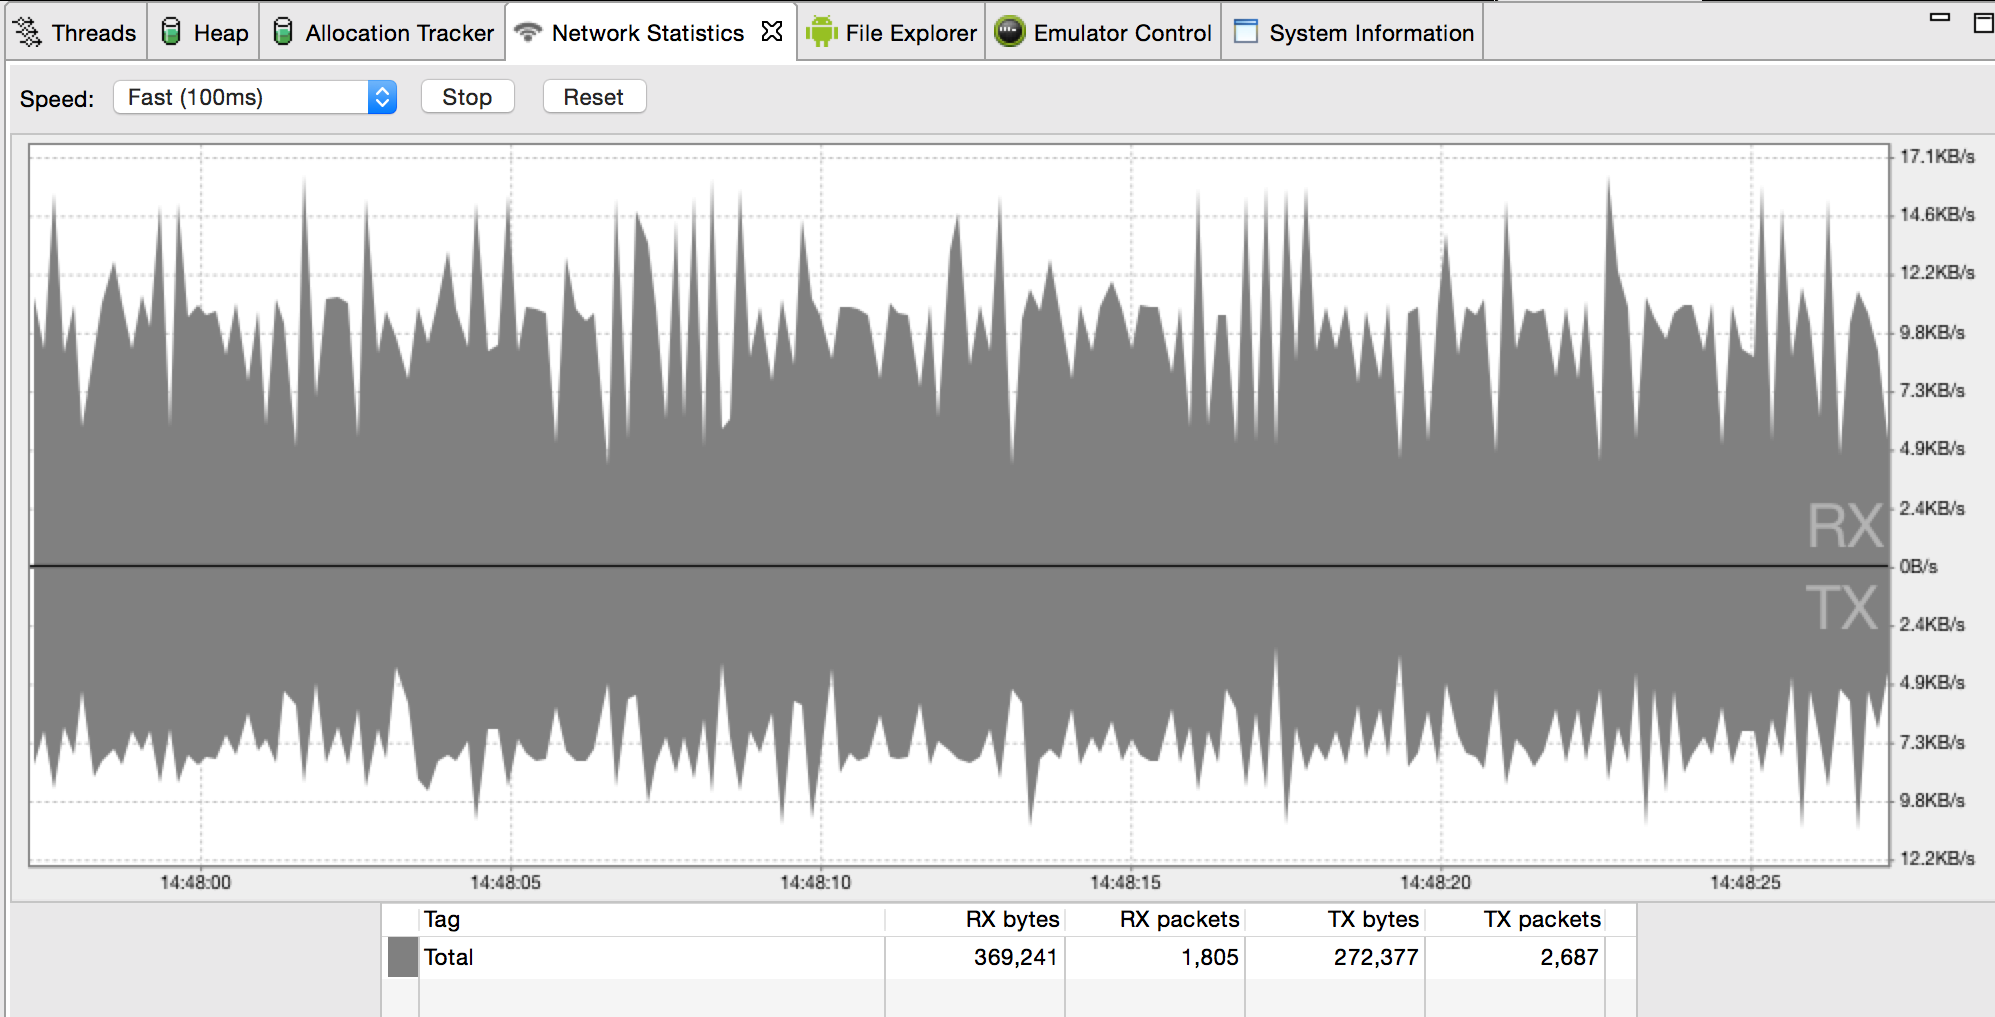
\includegraphics[width=0.8\textwidth]{images/ddms.png}
	\end{center}
	\caption{The DDMS tool from the Android Studio IDE used in the data usage analysis}
	\label{fig:ddms}
\end{figure} 

\subsection{Data usage}
\label{sec:data_usage}
We analyze the amount of data sent and received by the mobile control application during different tasks. Using the DDMS \footnote{Dalvik Debug Monitor Server} tool from Android Studio we were able to measure sent and received bytes by our application. The results for the different tasks are shown in the table below. \\

\begin{threeparttable}[htbp]
	\centering
	\begin{tabular}{ l | r r }
		\toprule
		Task	& Bytes received	& Bytes sent \\
		\midrule
		1) Add a new room to the residence				& 897		& 544 \\
		2) Add a new thermostat to a room				& 25'597		& 18'911 \\
		3) Add a new heating schedule entry				& 1'548		& 1'678 \\
		4) Delete a room							& 435		& 423 \\
		5) Delete a thermostat						& 435		& 444 \\
		6) Regular update\tnote{\textdagger}								& 136'952		& 26'315 \\
		7) Create the whole residence\tnote{\textdagger}					& 405'454  	& 299'133\\
		\bottomrule
	\end{tabular}
	\begin{tablenotes}
		\footnotesize{
			\item[\textdagger] The analysis was done using a residence consisting of ten rooms, each equipped with three thermostats.
		}
	\end{tablenotes}
	\caption{Results of data usage analysis.}
	\label{table:data_usage}
\end{threeparttable}

Tasks only adding or removing one element to or from the system require only between 0.5 and 1.5 kilobytes of data sent/received. The only exception to this is adding a new thermostat, but this is because on the server infrastructure, every thermostat has a heating schedule, hence when creating a new thermostat, we also need to add the whole heating schedule of the associated room to it. That's why task 2 goes up to 25 kilobytes of data received and about 19 kilobytes sent. 

The more interesting task is the regular update mentioned in Section \ref{sec:updates}, since this task runs every 15 minutes. As we can see with a very large residence of ten rooms each having three thermostats, updating the whole database still only requires about 136 kilobytes of data to be received and much less to be sent.

As a reference, we added task 7 to the table which is the creation of all the rooms and thermostats at once, since this was just a dummy residence with fake elements in it. Here the data sent and received is increased by a lot because of all the thermostats that needed to be added.

Evaluating the data above we can conclude that adding a thermostat requires the most data in both receiving and sending because of the heating table being set up.

\subsection{User study}
We have conducted a user study with 10 of our fellow students. After giving a brief introduction about the purpose and goal of the application to the participants, we first asked them to try to navigate through the different views of the app. Afterwards they were given a short list of tasks like creating a new room or deleting a thermostat. Each participant was motivated to take note of things that seemed uncomfortable or not intuitive.

For this user study the application was set up in such a way that it is possible to register a dummy residence with a fake RFID. Once registered, the application would automatically add 10 new rooms with randomly chosen but more or less sensible names and add two to four thermostats to each of them. Each thermostat was given an initial dummy value as its current temperature. This was done to be able to collect data for the user study in the case of users which have already set up the system. Some of the tasks also required rooms or thermostats to be already in the system. Of course for the tasks which involved adding new thermostats to the system, actual thermostats were provided with the NFC tags attached to them.

Half of the participants used smart phones not equipped with an NFC adapter for scanning the tags, so they were forced to use the manual entry of RFIDs for the study.

\subsection{Rating}
\label{sec:rating}
After the participants have successfully completed all their tasks, they were asked a series of questions to be answered on a scale of one through five with the following meaning:
\begin{itemize}
\item{1 - Very Bad}
\item{2 - Bad}
\item{3 - Average}
\item{4 - Good}
\item{5 - Very Good}
\end{itemize}

\subsection{Results}
The questions were all phrased in such a way that the scale of Section \ref{sec:rating} was applicable to the question. So most of the questions started with "How well were you able to" and continued from there as follows:
\begin{itemize}
\item{...navigate through the different views of the application?}

8 participants answered with "Very Good", the other two replied with "Good".
\item{...tell the difference between the different views?}

This question focused on designing the views visually in such a way that the user will not get lost while trying to find the feature he is looking for.

All 10 participants answered with "Very Good". 
\item{...quickly see the temperature of any given room and whether it's being heated up or not?}

All 10 participants answered with "Very Good".
\item{...change tomorrow's schedule for a given room?}

6 participants answered with "Very Good", three with "Good" and one "Average".

The biggest problem was figuring out that the schedule of a room could only be changed by going to the settings menu in the room's detail view. Having reached the schedule view for the room most participants were able to complete the task very easily.

\item{...delete a thermostat from a given room?}

All 10 participants answered with "Very Good".
\item{...delete a room from the system?}

All 10 participants answered with "Very Good".
\item{...add a thermostat to a given room?}

5 participants answered with "Very Good", two with "Good" and three with "Average".

All of the participants using a smart phone with a NFC adapter replied with "Very Good" since scanning the tag is very convenient for the user. The manual method still works, but it is rather cumbersome to be able to read the RFID written on the tags.
\item{...add a room to the system?}

All 10 participants answered with "Very Good".

\item{How would you rate the overall impression of the application visually?}

Two participants answered with "Very Good", 4 with "Good" and 4 with "Average".

\item{How would you rate the overall usability of the application?}

8 participants answered with "Very Good", two replied with "Good".

\item{Would you consider using such a heating system in your own home?}

Here the answers were not given in the usual scale but rather as statements. 

Most of the participants considered it not worth the price of exchanging all their thermostats at home and buying a raspberry pi just to maybe save a little bit of money in heating cost. These statements are of course from students which is probably not the best group for such a question, but conducting a bigger user study or even reaching out to users of existing smart heating systems for a questionnaire lies beyond the scope of this project.
\end{itemize}
